%% Thinking Forth
%% Copyright (C) 2004 Leo Brodie
%% Initial transcription by Nils M Holm
%% Based on OCR scans by John Hogerhuis
%% 
%% Chapter: Four - Detailed Design/Problem Solving

%!! horizontal line
%FOUR
%!! horizontal line

\chapter{Detailed~Design/\penalty 0\allowhyphens Problem~Solving}

\begin{tfquot}
\emph{Trivial:} I can see how to do this. I just don't know how long it
will take.\\
\emph{Non-trivial:} I haven't a \emph{clue} how to do this!

%!! right-justify paragraph
\begin{flushright}
---\emph{Operating philosophy developed at the Laboratory
Automation and Instrumentation Design Group,
Chemistry Dept., Virginia Polytechnic Institute and State University}
\end{flushright}
\end{tfquot}

Once you've decided upon the components in your application, your next
step is to design those components. In this chapter we'll apply
problem-solving techniques to the detailed design of a FORTH application.
This is the time for pure invention, the part that many of us find the most
fun. There's a special satisfaction in going to the mat with a non-trivial
problem and coming out the victor.

In English it's difficult to separate an idea from the words used to
express the idea. In writing a FORTH application it's difficult to
separate the detailed design phase from implementation, because we tend
to design in FORTH. For this reason, we'll get a bit ahead of ourselves in
this chapter by not only presenting a problem but also designing a solution
to it, right on through to the coded implementation.

\section{Problem-Solving Techniques}

Even neophytes can solve programming problems without devoting any
conscious thought to problem solving techniques. So what's the point in
studying techniques of problem solving? To quicken the process. By
thinking about the \emph{ways} in which we solve problems, apart from
the problems themselves, we enrich our subconscious storehouse of
techniques.

G. Polya has written several books on problem solving, especially of
the mathematical problem. The most accessible of these is \emph{How to Solve
It} [1]. Although solving a mathematical problem isn't quite the same as
solving a software problem, you'll find some valuable suggestions there.
The following series of tips summarize several techniques recommended by
the science of problem solving:
%!! horizontal line
\begin{tip}
Determine your goal.
\end{tip}
%!! horizontal line
Know what you're trying to accomplish. As we saw in Chapter Two, this
step can be detailed further:

Determine the data interfaces: Know what data will be required to
accomplish the goal, and make sure those data are available (input).
Know what data the function is expected to produce (output). For a single
definition, this means writing the stack-effect comment.

Determine the rules; review all the facts that you know. In Chapter
Two we described the rates for computing the cost of a phone call along
with the rules for applying the rates.
%!! horizontal line
\begin{tip}
Picture the problem as a whole.
\end{tip}
%!! horizontal line
In the \emph{analysis} phase we separated the problem into its parts, to
clarify our understanding of each piece. We are now entering the
\emph{synthesis} phase. We must visualize the problem as a whole.

Try to retain as much information about the problem in your mind
as possible. Use words, phrases, figures and tables, or any kind of graphic
representation of the data and/or rules to help you see the maximum
information at a glance. Fill your mind to bursting with the requirements
of the problem you need to solve, the way you might fill your lungs with
air.

Now hold that mental image, the way you might hold your breath.

One of two things will happen:

You may see the solution in a flash of insight. Great! Exhale a sigh
of relief and proceed directly to implementation. Or\dots{}, the problem is
too complex or too unfamiliar to be solved so easily. In this case, you'll
have to turn your attention to analogies and partial solutions. As you do
so, it's important that you have already concentrated on the problem's
requirements all at once, engraving these requirements on your mental
retina.
%!! horizontal line
\begin{tip}
Develop a plan.
\end{tip}
%!! horizontal line
If the solution didn't come at a glance, the next step is to determine the
approach that you will take to solve it. Set a course for action and avoid
the trap of fumbling about aimlessly.

The following tips suggest several approaches you might consider.
%!! horizontal line
\begin{tip}
Think of an analogous problem.
\end{tip}
%!! horizontal line
Does this problem sound familiar? Have you written a definition like it
before? Figure out what parts of the problem are familiar, and in what
ways this problem might differ. Try to remember how you solved it
before, or how you solved something like it.
%!! horizontal line
\begin{tip}
Work forward.
\end{tip}
%!! horizontal line
The normal, obvious way to attack a problem is by begining with the
known, and proceeding to the unknown. In deciding which horse to bet
on, you'd begin with their recent histories, their current health, and so on,
apply weights to these various factors and arrive at a favorite.
%!! horizontal line
\begin{tip}
Work backward.
\end{tip}
%!! horizontal line
More complicated problems present many possible ways to go with the
incoming data. How do you know which route will take you closer to the
solution? You don't. This class of problem is best solved by working
backward (\Fig{fig4-1}).

\wepsfiga{fig4-1}{A problem that is easier to solve backward than
forward.}

%!! include Figure 4-1 here

%!! horizontal line
\begin{tip}
Believe.
\end{tip}
%!! horizontal line
Belief is a necessary ingredient for successfully working backward. We'll
illustrate with a famous mathematical problem. Suppose we have two
containers. The containers have no graduation marks, but one holds nine
gallons and the other holds four gallons. Our task is to measure out exactly
six gallons of water from the nearby stream in one of the containers
(\Fig{fig4-2}).

\wepsfigt{fig4-2}{Two containers.}

%!! include Figure 4-2 here


Try to solve this on your own before reading further.

How can we get a ``six'' out of a ``nine'' and a ``four''? We can start
out working forward, by mentally transferring water from one container
to the other. For example, if we fill the large container twice from the
small container, we'll get eight gallons. If we fill the nine-gallon container
to the brim, then empty enough water to fill the four-gallon container,
we'll have exactly five gallons in the large container.

These ideas are interesting, but they haven't gotten us six gallons.
And it's not clear how they will get us six gallons.

Let's try working backward. We assume we've measured six gallons
of water, and it's sitting in the large container (it won't fit in the
small one!). Now, how did we get it there? What was the state of our
containers one step previously?

There are only two possibilities (\Fig{fig4-3}):
%!! there's certainly some better way to do ordered lists in TeX
\begin{enumerate}
\item The four-gallon container was full, and we just added it to the large
   container. This implies that we already had two gallons in the large
   container.
%!! line break?

   Or\dots{}
\item The nine gallon container was full, and we just poured off three gallons
   into the small container.
\end{enumerate}
Which choice? Let's make a guess. The first choice requires a two-gallon
measurement, the second requires a three-gallon measurement. In our initial
playing around, we never saw a unit like two. But we did see a difference
of one, and one from four is three. Let's go with version b.

Now comes the real trick. We must make ourselves \emph{believe} without
doubt that we have arrived at the situation described. We have just
poured off three gallons into the small container. Suspending all disbelief,
we concentrate on how we did it.

How can we pour off three gallons into the small container? If there
had already been one gallon in the small container! Suddenly we're over
the hump. The simple question now is, how do we get one gallon in the
small container? We must have started with a full nine-gallon container,
poured off four gallons twice, leaving one gallon. Then we transferred the
one gallon to the small container.

\wepsfigt{fig4-3}{Achieving the end result.}

%!! include Figure 4-3 here

%!! include cartoon of page 103 here

\wepsfigp{img4-103}{Intent on a complicated problem.}


Our final step should be to check our logic by running the problem
forwards again.

Here's another benefit of working backward: If the problem is unsolvable,
working backward helps you quickly prove that it has no solution.
%!! horizontal line
\begin{tip}
Recognize the auxiliary problem.
\end{tip}
%!! horizontal line
Before we've solved a problem, we have only a hazy notion of what
steps---or even how many steps---may be required. As we become more
familiar with the problem, we begin to recognize that our problem
includes one or more subproblems that somehow seem different from the
main outline of the proposed procedure.

In the problem we just solved, we recognized two subproblems: filling
the small container with one gallon and then filling the large container
with six gallons.

Recognizing these smaller problems, sometimes called ``auxiliary
problems,'' is an important problem-solving technique. By identifying
the subproblem, we can assume it has a straightforward solution.
Without stopping to determine what that solution might be, we forge
ahead with our main problem.

(FORTH is ideally suited to this technique, as we'll see.)
%!! horizontal line
\begin{tip}
Step back from the problem.
\end{tip}
%!! horizontal line
It's easy to get so emotionally attached to one particular solution that we
forget to keep an open mind.

The literature of problem solving often employs the example of the
nine dots. It stumped me, so I'll pass it along. We have nine dots arranged
as shown in \Fig{fig4-4}. The object is to draw straight lines that
touch or pass through all nine dots, without lifting the pen off the paper.
The constraint is that you must touch all nine dots with only four lines.

\wepsfiga{fig4-4}{The nine dots problem.}

%!! include Figure 4-4 here

You can sit a good while and do no better than the almost-right
\Fig{fig4-5}. If you concentrate really hard, you may eventually conclude
that the problem is a trick---there's no solution.

\wepsfiga{fig4-5}{Not quite right.}

%!! include Figure 4-5 here

But if you sit back and ask yourself,
%!! indent paragraph
\begin{tfquot}
``Am I cheating myself out a useful tack by being narrow-minded? Am I
assuming any constraints not specified in the problem? What constraints
might they be?''
\end{tfquot}
then you might think of extending some of the lines beyond the perimeter
of the nine dots.
%!! horizontal line
\begin{tip}
Use whole-brain thinking.
\end{tip}
%!! horizontal line
When a problem has you stumped and you seem to be getting nowhere,
relax, stop worrying about it, perhaps even forget about it for a while.

Creative people have always noted that their best ideas seem to
come out of the blue, in bed or in the shower. Many books on problem
solving suggest relying on the subconscious for the really difficult
problems.

Contemporary theories on brain functions explore the differences
between rational, conscious thought (which relies on the manipulation of
symbols) and subconscious thought (which correlates perceptions to
previously stored information, recombining and relinking knowledge in
new and useful ways).

Leslie Hart [2] explains the difficulty of solving a large problem by
means of logic:

%!! begin indented paragraph
\begin{tfquot}
A huge load is placed on that one small function of the brain that can be
brought into the attention zone for a period. The feat is possible, like the
circus act, but it seems more sensible to\dots{} use the full resources of our
glorious neocortex\dots{} the multibillion-neuron capacity of the brain.

\dots{} The work aspect lies in providing the brain with raw input, as in
observing, reading, collecting data, and reviewing what others have achieved.
Once in, [subconscious] procedures take over, simultaneously, automatically,
outside of the attention zone.

\dots{} It seems apparent\dots{} that a search is going on during the interval,
though not necessarily continuously, much as in a large computer. I would
hazard the guess that the search ramifies, starts and stops, reaches dead
ends and begins afresh, and eventually assembles an answer that is
evaluated and then popped into conscious attention---often in astonishingly
full-blown detail.
\end{tfquot}
%!! end indented paragraph
%!! horizontal line
\begin{tip}
Evaluate your solution. Look for other solutions.
\end{tip}
%!! horizontal line
You may have found one way of skinning the cat. There may be other
ways, and some of them may be better.

Don't invest too much effort in your first solution without asking
yourself for a second opinion.

%!! include cartoon of page 106 here
\wepsfigp{img4-106}{``I'm not just sleeping. I'm using my neocortex.''}

\section{Interview with a Software Inventor}

%!! horizontal line
\blackline{2ex}
Donald A. Burgess, owner and president of Scientek Instrumentation,
Inc.:

%!! begin indented paragraph
\begin{tfquot}
I have a few techniques I've found useful over the years in designing
anything, to keep myself flexible. My first rule is, ``Nothing is impossible.''
My second rule is, ``Don't forget, the object is to make a buck.''

First examine the problem, laying out two or three approaches on paper.
Then try the most appealing one, to see if it works. Carry it through. Then
deliberately go all the way back to the beginning, and start over.

Starting over has two values. First, it gives you a fresh approach. You
either gravitate back to the way you started, or the way you started
gravitates toward the new way.

Second, the new approach may show all kinds of powerful possibilities. Now
you have a benchmark. You can look at both approaches and compare the
advantages of both. You're in a better position to judge.

Getting stuck comes from trying too hard to follow a single approach.
Remember to say, ``I want this kumquat crusher to be different. Let's
reject the traditional design as not interesting. Let's try some crazy
ideas.''

The best thing is to start drawing pictures. I draw little men. That keeps
it from looking like ``data'' and interfering with my thinking process. The
human mind works exceptionally well with analogies. Putting things in
context keeps you from getting stuck within the confines of any language,
even FORTH.

When I want to focus my concentration, I draw on little pieces of paper.
When I want to think in broad strokes, to capture the overall flow, I draw
on great big pieces of paper. These are some of the crazy tricks I use to keep
from getting stagnant.

When I program in FORTH, I spend a day just dreaming, kicking around
ideas. Usually before I start typing, I sketch it out in general terms. No
code, just talk. Notes to myself.

Then I start with the last line of code first. I describe what I would like
to do, as close to English as I can. Then I use the editor to slide this
definition towards the bottom of the screen, and begin coding the internal
words. Then I realize that's a lousy way to do it. Maybe I split my top word
into two and transfer one of them to an earlier block so I can use it earlier.
I run the hardware if I have it; otherwise I simulate it.

FORTH requires self-discipline. You have to stop diddling with the
keyboard. FORTH is so willing to do what I tell it to, I'll tell it to do all
kinds of ridiculous things that have nothing to do with where I'm trying to
go. At those times I have to get away from the keyboard.

FORTH lets you play. That's fine, chances are you'll get some ideas. As
long as you keep yourself from playing as a habit. Your head is a whole lot
better than the computer for inventing things.
\end{tfquot}
\blackline{1ex}
%!! end indented paragraph
%!! horizontal line

{\othersidetrue\section{Detailed Design}}

We're now at the point in the development cycle at which we've decided
we need a component (or a particular word). The component will consist
of a number of words, some of which (those that comprise the lexicon) will
be used by other components and some of which (the internal words) will
be only used within this component.

Create as many words as necessary to obey the following tip:
%!! horizontal line
\begin{tip}
Each definition should perform a simple, well-defined task.
\end{tip}
%!! horizontal line
Here are the steps generally involved in designing a component:
%!! there's certainly some better way to do ordered lists in TeX
\begin{enumerate}
\item Based on the required functions, decide on the names and syntax for the
   external definitions (define the interfaces).
\item Refine the conceptual model by describing the algorithm(s) and data
   structure(s).
\item Recognize auxiliary definitions.
\item Determine what auxiliary definitions and techniques are already available.
\item Describe the algorithm with pseudocode,
\item Implement it by working backwards from existing definitions to the inputs,
\item Implement any missing auxiliary definitions.
\item If the lexicon contains many names with strong elements in common,
   design and code the commonalities as internal definitions, then implement
   the external definitions.
\end{enumerate}
We'll discuss the first two steps in depth. Then we'll engage in an
extended example of designing a lexicon.

\section{FORTH Syntax}

At this point in the development cycle you must decide how the words in
your new lexicon will be used in context. In doing so, keep in mind how
the lexicon will be used by subsequent components.
%!! horizontal line
\begin{tip}
In designing a component, the goal is to create a lexicon that will make your
later code readable and easy to maintain.
\end{tip}
%!! horizontal line
Each component should be designed with components that use it in mind.
You must design the syntax of the lexicon so that the words make sense
when they appear in context. Hiding interrelated information within the
component will ensure maintainability, as we've seen.
At the same time, observe FORTH's own syntax. Rather than insisting
on a certain syntax because it seems familiar, you may save
yourself from writing a lot of unnecessary code by choosing a syntax that
FORTH can support without any special effort on your part.

Here are some elementary rules of FORTH's natural syntax:
%!! horizontal line
\begin{tip}
Let numbers precede names.
\end{tip}
%!! horizontal line
%!! include cartoon of page 110 here
Words that require a numeric argument will naturally expect to find that
number on the stack. Syntactically speaking, then, the number should
precede the name. For instance, the syntax of the word \textbf{SPACES}, which
emits ``n'' number of spaces, is

\begin{Code}
20 SPACES
\end{Code}

Sometimes this rule violates the order that our ear is accustomed to
hearing. For instance, the FORTH word \textbf{+} expects to be preceded by both
arguments, as in

\begin{Code}
3 4 +
\end{Code}

This ordering, in which values precede operators, is called ``postfix.''
FORTH, in its magnanimity, won't \emph{insist} upon postfix notation.
You could redefine \textbf{+} to expect one number in the input stream, like this:

\begin{Code}
3 + 4
\end{Code}

by defining it so:
\begin{Code}
: +   BL WORD  NUMBER DROP  + ;
\end{Code}
(where \textbf{WORD} is 79/83 Standard, returning an address, and \textbf{NUMBER}
returns a double-length value as in the 83 Standard Uncontrolled
Reference Words).

Fine. But you wouldn't be able to use this definition inside other
colon definitions or pass it arguments, thereby defeating one of FORTH's
major advantages.

Frequently, ``noun'' type words pass their addresses (or any type of
pointer) as a stack argument to ``verb'' type words. The FORTH-like syntax of
\begin{quote}
%!! sans-serif
{\sf ``noun'' ``verb''}
\end{quote}
\wepsfigxx{img4-110}
will generally prove easiest to implement because of the stack.
In some cases this word order sounds unnatural. For instance, suppose
we have a file named INVENTORY. One thing we can do with that
file is SHOW it; that is, format the information in pretty columns. If

INVENTORY passes a pointer to SHOW, which acts upon it, the syntax
becomes
\begin{Code}
INVENTORY SHOW
\end{Code}
If your spec demands the English word-order, FORTH offers ways to
achieve it. But most involve new levels of complexity. Sometimes the
best thing to do is to choose a better name. How about
\begin{Code}
INVENTORY REPORT
\end{Code}
(We've made the ``pointer'' an adjective, and the ``actor'' a noun.)

If the requirements insist on the syntax
\begin{Code}
SHOW INVENTORY
\end{Code}
we have several options. SHOW might set a flag and INVENTORY
would act according to the flag. Such an approach has certain disadvantages,
especially that INVENTORY must be ``smart'' enough to
know all the possible actions that might be taken on it. (We'll treat these
problems in Chapters Seven and Eight.)

Or, SHOW might look ahead at the next word in the input stream.
We'll discuss this approach in a tip, ``Avoid expectations,'' later in this
chapter.

Or, the recommended approach, SHOW might set an ``execution
variable'' that INVENTORY will then execute. (We'll discuss vectored
execution in Chapter Seven.)
%!! horizontal line
\begin{tip}
Let text follow names.
\end{tip}
%!! horizontal line
If the FORTH interpreter finds a string of text that is neither a number
nor a predefined word, it will abort with an error message. For this
reason, an undefined string must be preceded by a defined word.

An example is \textbf{."} (dot-quote), which precedes the text it will later
print. Another example is \textbf{CREATE} (as well as all defining words), which
precedes the name that is, at the moment, still undefined.

The rule also applies to defined words that you want to refer to, but
not execute in the usual way. An example is \textbf{FORGET}, as in

\begin{Code}
FORGET TASK
\end{Code}

Syntactically, \textbf{FORGET} must precede TASK so that TASK doesn't
execute.
%!! horizontal line
\begin{tip}
Let definitions consume their arguments.
\end{tip}
%!! horizontal line
This syntax rule is more a convention of good FORTH programming
than a preference of FORTH.

Suppose you're writing the word LAUNCH, which requires the
number of a launch pad and fires the appropriate rocket. You want the
definition to look roughly like this:
\begin{Code}
: LAUNCH  ( pad#)  LOAD  AIM  FIRE ;
\end{Code}
Each of the three internal definitions will require the same argument, the
launch pad number. You'll need two \textbf{DUP}s somewhere. The question is
where? If you put them inside LOAD and AIM, then you can keep them
out of LAUNCH, as in the definition above. If you leave them out of
LOAD and AIM, you'll have to define:
\begin{Code}
: LAUNCH  ( pad#)  DUP LOAD  DUP AIM  FIRE ;
\end{Code}
By convention, the latter version is preferable, because LOAD and AIM
are cleaner. They do what you expect them to do. Should you have to
define READY, you can do it so:
\begin{Code}
: READY  ( pad#)  DUP LOAD  AIM ;
\end{Code}
and not
\begin{Code}
: READY  ( pad#)  LOAD  AIM  DROP ;
\end{Code}
%!! horizontal line
\begin{tip}
Use zero-relative numbering.
\end{tip}
%!! horizontal line
By habit we humans number things starting with one: ``first, second,
third,'' etc. Mathematical models, on the other hand, work more naturally
when starting with zero. Since computers are numeric processors, software
becomes easier to write when we use zero-relative numbering.

To illustrate, suppose we have a table of eight-byte records. The
first record occupies the first eight bytes of the table. To compute its
starting address, we add ``0'' to TABLE. To compute the starting address
of the ``second'' record, we add ``8'' to TABLE.

\wepsfiga{fig4-6}{A table of 8-byte records.}

%!! include Figure 4-6 here

It's easy to derive a formula to achieve these results:
%!! should be two columns, right-hand side sans-serif

\bigskip
\begin{tabular}{@{}l@{ }l@{}r}
\sf first record starts at:  &  $\mathsf{0 \times 8} = {}$ & \sf 0  \\
\sf second record starts at: &  $\mathsf{1 \times 8} = {}$ & \sf 8  \\
\sf third record starts at:  &  $\mathsf{2 \times 8} = {}$ & \sf 16 \\
\end{tabular}
\bigskip

We can easily write a word which converts a record\# into the address
where that record begins:

\begin{Code}
: RECORD  ( record# -- adr )
   8 *  TABLE + ;
\end{Code}

Thus in computer terms it makes sense to call the ``first record'' the Oth
record.

If your requirements demand that numbering start at one, that's
fine. Use zero-relative numbering throughout your design and then, only
in the ``user lexicons'' (the set of words that the end-user will use)
include the conversion from zero-to one-relative numbering:
\begin{Code}
: ITEM  ( n -- adr)  1- RECORD ;
\end{Code}
%!! horizontal line
\begin{tip}
Let addresses precede counts.
\end{tip}
%!! horizontal line
Again, this is a convention, not a requirement of FORTH, but such conventions
are essential for readable code. You'll find examples of this rule
in the words \textbf{TYPE}, \textbf{ERASE}, and \textbf{BLANK}.
%!! horizontal line
\begin{tip}
Let sources precede destinations.
\end{tip}
%!! horizontal line
Another convention for readability. For instance, in some systems, the
phrase
\begin{Code}
22 37 COPY
\end{Code}
copies Screen 22 to Screen 37. The syntax of CMOVE incorporates both
this convention and the previous convention:
%!! does \bf work inside verbatim blocks?
\begin{Code}[commandchars=\&\{\}]
source destination count &poorbf{CMOVE}
\end{Code}
%!! horizontal line
\begin{tip}
Avoid expectations (in the input stream).
\end{tip}
%!! horizontal line
Generally try to avoid creating words that presume there will be other
words in the input stream.

Suppose your color computer represents blue with the value 1, and
light-blue with 9. You want to define two words: BLUE will return 1;
LIGHT may precede BLUE to produce 9.

In FORTH, it would be possible to define BLUE as a constant, so
that when executed it always returns 1.

\begin{Code}
1 CONSTANT BLUE
\end{Code}

And then define LIGHT such that it looks for the next word in the input
stream, executes it, and ``ors'' it with 8 (the logic of this will become
apparent when we visit this example again, later in the book):
\begin{Code}
: LIGHT  ( precedes a color)  ( -- color value)
     ' EXECUTE  8 OR ;
\end{Code}
(in fig-FORTH:
\begin{Code}
: LIGHT [COMPILE] '  CFA EXECUTE  8 OR ;)
\end{Code}
%!! The closing paren at the end of this code is a bit misleading.
%!! At least a leading space and a different font should be used.
(For novices: The apostrophe in the definition of LIGHT is a FORTH
word called ``tick.'' Tick is a dictionary-search word; it takes a name and
looks it up in the dictionary, returning the address where the definition
resides. Used in this definition, it will find the address of the word
following LIGHT---for instance, BLUE---and pass this address to the word
\textbf{EXECUTE}, which will execute BLUE, pushing a one onto the stack.
Having ``sucked up'' the operation of BLUE, LIGHT now ``or''s an 8 into
the 1, producing a 9.)

This definition will work when invoked in the input stream, but special
handling is required if we want to let LIGHT be invoked within a
colon definition, as in:
\begin{Code}
: EDITING   LIGHT BLUE BORDER ;
\end{Code}
Even in the input stream, the use of EXECUTE here will cause
a crash if LIGHT is accidentally followed by something other than a
defined word.  The preferred technique, if you're forced to use this
particular syntax, is to have LIGHT set a flag, and have BLUE
determine whether that flag was set, as we'll see later on.

There will be times when looking ahead in the input stream is desirable,
even necessary. (The proposed TO solution is often implemented
this way [3].)

But generally, avoid expectations. You're setting yourself up for
disappointment.

%!! horizontal line
\begin{tip}
Let commands perform themselves.
\end{tip}
%!! horizontal line

This rule is a corollary to ``Avoid expectations.'' It's one of
FORTH's philosophical quirks to let words do their own work. Witness
the FORTH compiler (the function that compiles colon definitions),
carcicatured in \Fig{fig4-7}. It has very few rules:

\wepsfigt{fig4-7}{The traditional compiler vs. the FORTH compiler.}

%!! include Figure 4-7 here

%!! this paragraph should be an indented, unordered list
\begin{tfquot}
Scan for the next word in the input stream and look it up in the dictionary.

If it's an ordinary word, \emph{compile} its address.

If it's an ``immediate'' word, \emph{execute} it.

If it's not a defined word, try to convert it to a number and compile it as a
literal.

If it's not a number, abort with an error message.
\end{tfquot}
Nothing is mentioned about compiling-words such as \textbf{IF}, \textbf{ELSE},
\textbf{THEN}, etc. The colon compiler doesn't know about these words. It merely
recognizes certain words as ``immediate'' and executes them, letting
them do their own work. (See \emph{Starting FORTH}, Chapter Eleven, ``How to
Control the Colon Compiler.'')

The compiler doesn't even ``look for'' semicolon to know when to
stop compiling. Instead it executes semicolon, allowing it to do the work
of ending the definition and shutting off the compiler.

There are two tremendous advantages to this approach. First, the
compiler is so simple it can be written in a few lines of code. Second,
there's no limit on the number of compiling words you can add at any
time, simply by making them immediate. Thus, even FORTH's colon
compiler is extensible!

FORTH's text interpreter and FORTH's address interpreter also
adhere to this same rule.

The following tip is perhaps the most important in this chapter:

%!! horizontal line
\begin{tip}
Don't write your own interpreter/compiler when you can use FORTH's.
\end{tip}
%!! horizontal line
One class of applications answers a need for a special purpose
language---a self-contained set of commands for doing one particular
thing. An example is a machine-code assembler. Here you have a large
group of commands, the mnemonics, with which you can describe the
instructions you want assembled. Here again, FORTH takes a radical
departure from mainstream philosophy.

Traditional assemblers are special-purpose interpreters---that is,
they are complicated programs that scan the assembly-language listing
looking for recognized mnemonics such as ADD, SUB, JMP, etc., and
assemble machine instructions correspondingly. The FORTH assembler,
however, is merely a lexicon of FORTH words that themselves assemble
machine instructions.

There are many more examples of the special purpose language,
each specific to individual applications. For instance:

%!! begin ordered list
\begin{enumerate}
\item If you're building an Adventure-type game, you'd want to write a language
that lets you create and describe monsters and rooms, etc. You might
create a defining word called ROOM to be used like this:

\begin{Code}
ROOM DUNGEON
\end{Code}

Then create a set of words to describe the room's attributes by building
unseen data structures associated with the room:

\begin{Code}
EAST-OF DRAGON-LAIR
WEST-OF BRIDGE
CONTAINING POT-O-GOLD
etc.
\end{Code}
%!! 'etc.' should not be part of the code, should it?

The commands of this game-building language can simply be FORTH
WORDS, with FORTH as the interpreter.

\item If you're working with Programmable Array Logic (PAL) devices, you'd
like a form of notation that lets you describe the behavior of the output pins
in logical terms, based on the states of the input pins. A PAL programmer
was written with wonderful simplicity in FORTH by Michael Stolowitz [4].

\item If you must create a series of user menus to drive your application, you
might want to first develop a menu-compiling language. The words of this
new language allow an application programmer to quickly program the
needed menus---while hiding information about how to draw borders, move
the cursor, etc.
\end{enumerate}
All of these examples can be coded in FORTH as lexicons, using the normal
FORTH interpreter, without having to write a special-purpose interpreter
or compiler.

\bigskip
%!! horizontal line
\blackline{2ex}
Moore:

\begin{tfquot}
A simple solution is one that does not obscure the problem with irrelevancies.
It's conceivable that something about the problem requires a unique
interpreter. But every time you see a unique interpreter, it implies that
there is something particularly awkward about the problem. And that is
almost never the case.

If you write your own interpreter, the interpreter is almost certainly the
most complex, elaborate part of your entire application. You have switched
from solving a problem to writing an interpreter.

I think that programmers like to write interpreters. They like to do these
elaborate difficult things. But there comes a time when the world is going
to have to quit programming keypads and converting numbers to binary,
and start solving problems.
\end{tfquot}
\blackline{1ex}
%!! horizontal line

\section{Algorithms and Data Structures}

In Chapter Two we learned how to describe a problem's requirements in
terms of interfaces and rules. In this section we'll refine the conceptual
model for each component into clearly defined algorithms and data
structures.

An algorithm is a procedure, described as a finite number of rules,
for accomplishing a certain task. The rules must be unambiguous and
guaranteed to terminate after a finite number of applications. (The word
is named for the ninth century Persian mathematician al-Khowarizimi.)

An algorithm lies halfway between the imprecise directives of
human speech, such as ``Please sort these letters chronologically,'' and the
precise directives of computer language, such as ``BEGIN 2DUP < IF \dots{}''
etc. The algorithm for sorting letters chronologically might be this:
%!! there's certainly some better way to do ordered lists in TeX
\begin{enumerate}
\item Take an unsorted letter and note its date.
\item Find the correspondence folder for that month and year.
\item Flip through the letters in the folder, starting from the front, until
   you find the first letter dated later than your current letter.
\item Insert your current letter just in front of the letter dated later.
   (If the folder is empty, just insert the letter.)
\end{enumerate}
There may be several possible algorithms for the same job. The algorithm
given above would work fine for folders containing ten or fewer letters,
but for folders with a hundred letters, you'd probably resort to a more
efficient algorithm, such as this:
\begin{enumerate}
\item (same)
\item (same)
\item If the date falls within the first half of the month, open the folder a
   third of the way in. If the letter you find there is dated later than your
   current letter, search forward until you find a letter dated the same or
   before your current letter. Insert your letter at that point. If the letter
   you find is dated earlier than your current letter, search backward\dots{}
\end{enumerate}
\dots{} You get the point. This second algorithm is more complicated than
the first. But in execution it will require fewer steps on the average
(because you don't have to search clear from the beginning of the folder
every time) and therefore can be performed faster.

A data structure is an arrangement of data or locations for data,
organized especially to match the problem. In the last example, the file
cabinet containing folders and the folders containing individual letters
can be thought of as data structures.

The new conceptual model includes the filing cabinets and folders
(data structures) plus the steps for doing the filing (algorithms).

\section{Calculations vs. Data Structures vs. Logic}

We've stated before that the best solution to a problem is the simplest
adequate one; for any problem we should strive for the simplest
approach.

Suppose we must write code to fulfill this specification:

%!! sans-serif
\medskip
{\sf if the input argument is 1, the output is 10}

{\sf if the input argument is 2, the output is 12}

{\sf if the input argument is 3, the output is 14}

\medskip

There are three approaches we could take:

\emph{Calculation}

\begin{Code}
( n)  1-  2*  10 +
\end{Code}

\emph{Data Structure}

\begin{Code}
CREATE TABLE  10 C,  12 C,  14 C,
( n)  1- TABLE + C@
\end{Code}

\emph{Logic}

\begin{Code}
( n)  CASE
         1 OF 10 ENDOF
         2 OF 12 ENDOF
         3 OF 14 ENDOF  ENDCASE
\end{Code}
In this problem, calculation is simplest. Assuming it is also adequate
(speed is not critical), calculation is best.

The problem of converting angles to sines and cosines can be implemented
more simply (at least in terms of lines of code and object size)
by calculating the answers than by using a data structure. But for many
applications requiring trig, it's faster to look up the answer in a table
stored in memory. In this case, the simplest \emph{adequate} solution is using
the data structure.

In Chapter Two we introduced the telephone rate problem. In that
problem the rates appeared to be arbitrary, so we designed a data
structure:

\bigskip
%!! this shoulde be a table; see pg 119
\begin{tabular}{lccc}
          & \emph{Full Rate} & \emph{Lower Rate} & \emph{Lowest Rate} \\ \hline
First Min.  &       .30        &        .22        &          .12 \\ \hline
Add'1 Mins. &       .12        &        .10        &          .06 \\ \hline
\end{tabular}
\bigskip

Using a data structure was simpler than trying to invent a formula by
which these values could be calculated. And the formula might prove
wrong later. In this case, table-driven code is easier to maintain.

In Chapter Three we designed a keystroke interpreter for our Tiny
Editor using a decision table:

%!! this shoulde be a table; see pg 119
\begin{tabular}{lll}
\emph{Key}         & \emph{Not-Inserting} & \emph{Inserting} \\
\texttt{Cntrl-D}   & \texttt{DELETE}      & \texttt{INSERT-OFF} \\
\texttt{Cntrl-I}   & \texttt{INSERT-ON}   & \texttt{INSERT-OFF} \\
\texttt{backspace} & \texttt{BACKWARD}    & \texttt{INSERT<} \\
etc. & &
\end{tabular}

We could have achieved this same result with logic:

\begin{Code}
CASE
   CNTRL-D    OF  'INSERTING @  IF
      INSERT-OFF   ELSE DELETE     THEN   ENDOF
   CNTRL-I    OF  'INSERTING @  IF
      INSERT-OFF   ELSE INSERT-ON  THEN   ENDOF
   BACKSPACE  OF  'INSERTING @  IF
      INSERT<      ELSE BACKWARD   THEN   ENDDF
ENDCASE
\end{Code}
but the logic is more confusing. And the use of logic to express such a
multi-condition algorithm gets even more convoluted when a table was
not used in the original design.

The use of logic becomes advisable when the result is not calculable,
or when the decision is not complicated enough to warrent a decision
table. Chapter Eight is devoted to the issue of minimizing the use of logic
in your programs.

%!! horizontal line
\begin{tip}
In choosing which approach to apply towards solving a problem, give
preference in the following order:

%!! there's certainly some better way to do ordered lists in TeX
\begin{enumerate}
\item calculation (except when speed counts)
\item data structures
\item logic
\end{enumerate}
\end{tip}
%!! horizontal line
Of course, one nice feature of modular languages such as FORTH is that
the actual implementation of a component---whether it uses calculation,
data structures, or logic---doesn't have to be visible to the rest of the
application.

\section{Solving a Problem: Computing Roman Numerals}

In this section we'll attempt to demonstrate the process of designing a
lexicon. Rather than merely present the problem and its solution, I'm
hoping we can crack this problem together. (I kept a record of my
thought processes as I solved this problem originally.) You'll see
elements of the problem-solving guidelines previously given, but you'll
also see them being applied in a seemingly haphazard order---just as they
would be in reality.

Here goes: The problem is to write a definition that consumes a
number on the stack and displays it as a Roman numeral.

This problem most likely represents a component of a larger
system. We'll probably end up defining several words in the course of
solving this problem, including data structures. But this particular
lexicon will include only one name, ROMAN, and it will take its argument
from the stack. (Other words will be internal to the component.)

Having thus decided on the external syntax, we can now proceed to
devise the algorithms and data structures.

We'll follow the scientific method---we'll observe reality, model a
solution, test it against reality, modify the solution, and so on. We'll
begin by recalling what we know about Roman numerals.

Actually, we don't remember any formal rules about Roman
numerals. But if you give us a number, we can make a Roman numeral
out of it. We know how to do it---but we can't yet state the procedure as
an algorithm.

So, let's look at the first ten Roman numerals:

%!! paragraph should be sans-serif + indented
\bigskip
{\sf\begin{tabular}{r}
I \\
II \\
III \\
IV \\
V \\
VI \\
VII \\
VIll \\
IX \\
X \\
\end{tabular}}
\bigskip

\noindent We make a few observations. First, there's the idea of a
tally, where we represent a number by making that many marks (3 =
III). On the other hand, special symbols are used to represent groups
(5 = V). In fact, it seems we can't have more than three I's in a row
before we use a larger symbol.

Second, there's a symmetry around five. There's a symbol for five
(V), and a symbol for ten (X). The pattern I, II, III repeats in the second
half, but with a preceding V.

One-less-than-five is written IV, and one-less-than-ten is written IX.
It seems that putting an ``I'' in front of a larger-value symbol is like
saying ``one-less-than\dots{}''

These are vague, hazy observations. But that's alright. We don't
have the whole picture yet.

Let's study what happens above ten:

%!! paragraph should be sans-serif + indented
\bigskip
{\sf\begin{tabular}{r}
XI \\
XII \\
XIII \\
XIV \\
XV \\
XVI \\
XVII \\
XVIII \\
XIX \\
XX \\
\end{tabular}}

\noindent This is exactly the pattern as before, with an extra ``X''
in front. So there's a repeating cycle of ten, as well.

If we look at the twenties, they're the same, with two ``X''s; the
thirties with three ``X''s. In fact, the number of ``X'' is the same as the
number in the tens column of the original decimal number.

This seems like an important observation: we can decompose our decimal
number into decimal digits, and treat each digit separately. For instance,
37 can be written as

%!! sans-serif + indented
\begin{quote}
{\sf XXX (thirty)}
\end{quote}

\noindent followed by

%!! sans-serif + indented
\begin{quote}
{\sf VII (seven)}
\end{quote}

\noindent It may be premature, but we can already see a method by
which FORTH will let us decompose a number into decimal digits---with
modulo divison by ten. For instance, if we say

\begin{Code}
37 10 /MOD
\end{Code}
we'll get a 7 and a 3 on the stack (the three---being the quotient---is on
top.)

But these observations raise a question: What about below ten,
where there is no decimal digit? Is this a special case? Well, if we consider
that each ``X'' represents ten, then the absence of ``X'' represents zero.
So it's \emph{not} a special case. Our algorithm works, even for numbers less
than ten.

Let's continue our observations, paying special attention to the
cycles of ten. We notice that forty is ``XL.'' This is analogous to 4 being
``IV,'' only shifted by the value of ten. The ``X'' before the ``L'' says
``ten-less-than-fifty.'' Similarly,

%!! paragraph should be sans-serif + indented
\bigskip
{\sf\begin{tabular}{rrcrr}
   L &  (50) &   is analogous to &     V & (5) \\
  LX &  (60) &          "        &    VI & (6) \\
 LXX &  (70) &          "        &   VII & (7) \\
LXXX &  (80) &          "        &  VIII & (8) \\
  XC &  (90) &          "        &    IX & (9) \\
   C & (100) &          "        &     X & (10) \\
\end{tabular}}
\bigskip

Apparently the same patterns apply for any decimal digit---only the
symbols themselves change. Anyway, it's clear now that we're dealing with
an essentially decimal system.

If pressed to do so, we could even build a model for a system to display
Roman numerals from 1 to 99, using a combination of algorithm and
data structure.

{\othersidetrue\subsection{Data Structure}}

%!! see table on pg 123
\bigskip
\begin{tabular}{crccr}
\multicolumn{2}{c}{\underline{\emph{Ones' Table}}} &
\hbox to 3em{\hss} & \multicolumn{2}{c}{\underline{\emph{Tens' Table}}} \\
 0 &          & &     0 & \\
 1 &       I  & &     1 &      X \\
 2 &      II  & &     2 &     XX \\
 3 &     III  & &     3 &    XXX \\
 4 &      IV  & &     4 &     XL \\
 5 &       V  & &     5 &      L \\
 6 &      VI  & &     6 &     LX \\
 7 &     VII  & &     7 &    LXX \\
 8 &    VIII  & &     8 &   LXXX \\
 9 &      IX  & &     9 &     XC \\
\end{tabular}
\bigskip

\subsection{Algorithm}

Divide n by 10. The quotient is the tens' column digit; the remainder is
the ones' column digit. Look up the ten's digit in the tens' table and print
the corresponding symbol pattern. Look up the ones' digit in the one's
table and print that corresponding symbol pattern.

For example, if the number is 72, the quotient is 7, the remainder is
2. 7 in the tens' table corresponds to ``LXX,'' so print that. 2 in the ones'
column corresponds to ``II,'' so print that. The result:

%!! sans-serif + indented
\begin{quote}
{\sf LXXII}
\end{quote}
We've just constructed a model that works for numbers from one to 99.
Any higher number would require a hundreds' table as well, along with
an initial division by 100.

The logical model just described might be satisfactory, as long as it
does the job. But somehow it doesn't seem we've fully solved the problem.
We avoided figuring out how to produce the basic pattern by storing
all possible combinations in a series of tables. Earlier in this chapter we
observed that calculating an answer, if it's possible, can be easier than
using a data structure.

Since this section deals with devising algorithms, let's go all the
way. Let's look for a general algorithm for producing any digit, using
only the elementary set of symbols. Our data structure should contain
only this much information:

%!! sans-serif + indented
\bigskip
{\sf\begin{tabular}{c@{\hspace{1em}}c}
I & V \\
X & L \\
C & D \\
M & \\
\end{tabular}}
\bigskip

In listing the symbols, we've also \emph{organized} them in a way that seems
right. The symbols in the left column are all multiples of ten; the symbols
in the right column are multiples of five. Furthermore, the symbols in
each row have ten times the value of the symbols directly above them.

Another difference, the symbols in the first column can all be combined
in multiples, as ``XXXIII.'' But you can't have multiples of any of
the right-column symbols, such as VVV. Is this observation useful? Who
knows?

Let's call the symbols in the left column ONERS and in the right
column FIVERS. The ONERS represent the values 1, 10, 100, and 1,000;
that is, the value of one in every possible decimal place. The FIVERS
represent 5, 50, and 500; that is, the value of five in every possible
decimal place.

Using these terms, instead of the symbols themselves, we should be
able to express the algorithm for producing any digit. (We've factored
out the actual symbols from the \emph{kind} of symbols.) For instance, we can
state the following preliminary algorithm:

%!! indent paragraph
\begin{tfquot}
For any digit, print as many ONERS as necessary to add up to the value.
\end{tfquot}
Thus, for 300 we get ``CCC,'' for 20 we get ``XX'' for one we get ``I.'' And
for 321 we get ``CCCXXI.''

This algorithm works until the digit is 4. Now we'll have to expand
our algorithm to cover this exception:

%!! indent paragraph
\begin{tfquot}
Print as many ONERS as necessary to add up to the value, but if the digit
is 4, print a ONER then a FIVER.
%!! vertical half space
Hence, 40 is ``XL''; 4 is ``IV.''
\end{tfquot}
This new rule works until the digit is 5. As we noticed before, digits of
five and above begin with a FIVER symbol. So we expand our rule again:

%!! indent paragraph
\begin{tfquot}
If the digit is 5 or more, begin with a FIVER and subtract five from the
value; otherwise do nothing. Then print as many ONERS as necessary to
add up to the value. But if the digit is 4, print only a ONER and a FIVER.
\end{tfquot}
This rule works until the digit is 9. In this case, we must print a ONER
preceding a---what? A ONER from the next higher decimal place (the
next row below). Let's call this a TENER. Our complete model, then is:

%!! indent paragraph
\begin{tfquot}
If the digit is 5 or more, begin with a FIVER and subtract five from the
value; otherwise do nothing. Then, print as many ONERS as necessary to
add up to the value. But if the digit is 4, print only a ONER and a FIVER,
or if it's 9, print only a ONER and a TENER.
\end{tfquot}
We now have an English-language version of our algorithm. But we still
have some steps to go before we can run it on our computer.

In particular, we have to be more specific about the exceptions. We
can't just say,

%!! indent paragraph
\begin{tfquot}
Do a, b, and c. \emph{But} in such and such a case, do something different.
\end{tfquot}
because the computer will do a, b, and c before it knows any better.

Instead, we have to check whether the exceptions apply \emph{before} we
do anything else.

%!! horizontal line
\begin{tip}
In devising an algorithm, consider exceptions last. In writing code, handle
exceptions first.
\end{tip}
%!! horizontal line
This tells us something about the general structure of our digit-producing
word. It will have to begin with a test for the 4/9 exceptions. In
either of those cases, it will respond accordingly. If neither exception
applies, it will follow the ``normal'' algorithm. Using pseudocode, then:

\begin{Code}
: DIGIT  ( n )  4-OR-9? IF  special cases
   ELSE  normal case  THEN ;
\end{Code}

An experienced FORTH programmer would not actually write out this
pseudocode, but would more likely form a mental image of the structure
for eliminating the special cases. A less experienced programmer might
find it helpful to capture the structure in a diagram, or in code as we've
done here.

In FORTH we try to minimize our dependence on logic. But in this
case we need the conditional \textbf{IF} because we have an exception we need to
eliminate. Still, we've minimized the complexity of the control structure
by limiting the number of \textbf{IF THEN}s in this definition to one.

Yes, we still have to distinguish between the 4-case and the 9-case,
but we've deferred that structural dimension to lower-level
definitions---the test for 4-or-9 and the ``special case'' code.

What our structure really says is that either the 4-exception or the
9-exception must prohibit execution of the normal case. It's not enough
merely to test for each exception, as in this version:

\begin{Code}
: DIGIT  ( n )  4-CASE? IF  ONER FIVER  THEN
                9-CASE? IF  ONER TENER  THEN
                normal case... ;
\end{Code}

because the normal case is never excluded. (There's no way to put an
\textbf{ELSE} just before the normal case, because \textbf{ELSE} must appear between
\textbf{IF} and \textbf{THEN}.)

If we insist on handling the 4-exception and the 9-exception
separately, we could arrange for each exception to pass an additional
flag, indicating that the exception occurred. If either of these flags is
true, then we can exclude the normal case:

%!! warning: \textbf{} in verbatim block
\begin{Code}[commandchars=\&\{\}]
: DIGIT  ( n )  4-CASE? &poorbf{DUP} IF  ONER FIVER  THEN
                9-CASE? &poorbf{DUP} IF  ONER TENER  THEN
                OR  NOT IF normal case THEN ;
\end{Code}
But this approach needlessly complicates the definition by adding new
control structures. We'll leave it like it was.

Now we have a general idea of the structure of our main definition.
We stated, ``If the digit is 5 or more, begin with a FIVER and subtract
five from the value; otherwise do nothing. Then, print as many
ONERS as necessary to add up to the value.''

A direct translation of these rules into FORTH would look like this:

\begin{Code}
( n)  DUP  4 > IF  FIVER 5 -  THEN  ONERS
\end{Code}
This is technically correct, but if we're familiar with the technique of
modulo divison, we'll see this as a natural situation for modulo division
by 5. If we divide the number by five, the quotient will be zero (false)
when the number is less than five, and one (true) when it's between 5 and
9. We can use it as the boolean flag to tell whether we want the leading
FIVER:

\begin{Code}
( n )  5 / IF FIVER THEN ...
\end{Code}
The quotient/flag becomes the argument to IF.

Furthermore, the remainder of modulo 5 division is always a
number between 0 and 4, which means that (except for our exception) we
can use the remainder directly as the argument to ONERS. We revise our
phrase to

%!! warning: \textbf{} in verbatim block
\begin{Code}[commandchars=\&\{\}]
( n )  5 &poorbf{/MOD} IF FIVER THEN  &poorbf{ONERS}
\end{Code}
Getting back to that exception, we now see that we can test for both 4
and 9 with a single test---namely, if the remainder is 4. This suggests that
we can do our 5 \textbf{/MOD} first, then test for the exception. Something like
this:

%!! warning: \textbf{} in verbatim block
\begin{Code}[commandchars=\&\{\}]
: DIGIT  ( n )
     5 /MOD  &poorbf{OVER 4 =  IF  special case  ELSE}
     IF FIVER THEN  ONERS  THEN ;
\end{Code}
(Notice that we \textbf{OVER}ed the remainder so that we could compare it with
4 without consuming it.)

So it turns out we \emph{do} have a doubly-nested \textbf{IF THEN} construct
after all. But it seems justified because the \textbf{IF THEN} is handling the
special case. The other is such a short phrase, ``IF FIVER THEN'', it's
hardly worth making into a separate definition. You could though. (But we
won't.)

Let's focus on the code for the special case. To state its algorithm:
``If the digit is four, print a ONER and a FIVER. If the digit is nine, print
a ONER and a TENER.''

We can assume that the digit will be one or the other, or else we'd
never be executing this definition. The question is, how do we tell which
one?

Again, we can use the quotient of division by five. If the quotient is
zero, the digit must have been four; otherwise it was nine. So we'll play
the same trick and use the quotient as a boolean flag. We'll write:

\begin{Code}
: ALMOST  ( quotient )
     IF  ONER TENER  ELSE  ONER FIVER  THEN ;
\end{Code}
In retrospect, we notice that we're printing a ONER either way. We can
simplify the definition to:

\begin{Code}
: ALMOST  ( quotient )
     ONER  IF TENER ELSE FIVER THEN ;
\end{Code}
We've assumed that we have a quotient on the stack to use. Let's go back
to our definition of DIGIT and make sure that we do, in fact:

%!! warning: \textbf{} in verbatim block
\begin{Code}[commandchars=\&\{\}]
: DIGIT  ( n )
     5 /MOD  OVER 4 =  IF  &poorbf{ALMOST}  ELSE
     IF FIVER THEN  ONERS  THEN ;
\end{Code}
It turns out that we have not only a quotient, but a remainder
underneath as well. We're keeping both on the stack in the event we
execute the \textbf{ELSE} clause. The word \textbf{ALMOST}, however, only needs the
quotient. So, for symmetry, we must \textbf{DROP} the remainder like this:

%!! warning: \textbf{} in verbatim block
\begin{Code}[commandchars=\&\{\}]
: DIGIT  ( n )
     5 /MOD  OVER 4 =  IF  ALMOST  &poorbf{DROP}  ELSE
     IF FIVER THEN  ONERS  THEN ;
\end{Code}
There we have the complete, coded definition for producing a single digit
of a Roman numeral. If we were desperate to try it out before writing the
needed auxiliary definitions, we could very quickly define a lexicon of
words to print one group of symbols, say the ONES row:

%!! there is a small mistake in the original book:
%!! : TENER   ." X"; <-- missing space
%!! Fixed that.
\begin{Code}
: ONER    ." I" ;
: FIVER   ." V" ;
: TENER   ." X" ;
: ONERS  ( # of oners -- )
     ?DUP IF 0 DO  ONER  LOOP  THEN ;
\end{Code}
before loading our definitions of ALMOST and DIGIT.

But we're not that desperate. No, we're anxious to move on to the
problem of defining the words ONER, FIVER, and TENER so that their
symbols depend on which decimal digit we're formatting.

Let's go back to the symbol table we drew earlier:

%!! sans-serif + indented, heading in italics
\bigskip{\sf
\begin{tabular}{rll}
          & \it ONERs & \it FIVERs \\
     ones & I  &  V \\
     tens & X  &  L \\
 hundreds & C  &  D \\
thousands & M  & \\
\end{tabular}}
\bigskip

We've observed that we also need a ``TENER''---which is the ONER in
the next row below. It's as if the table should really be written:

%!! Here comes above table again, but this time with
%!! some circles and lines in it. I have no clue how
%!! to render this. See pg 128.
\bigskip
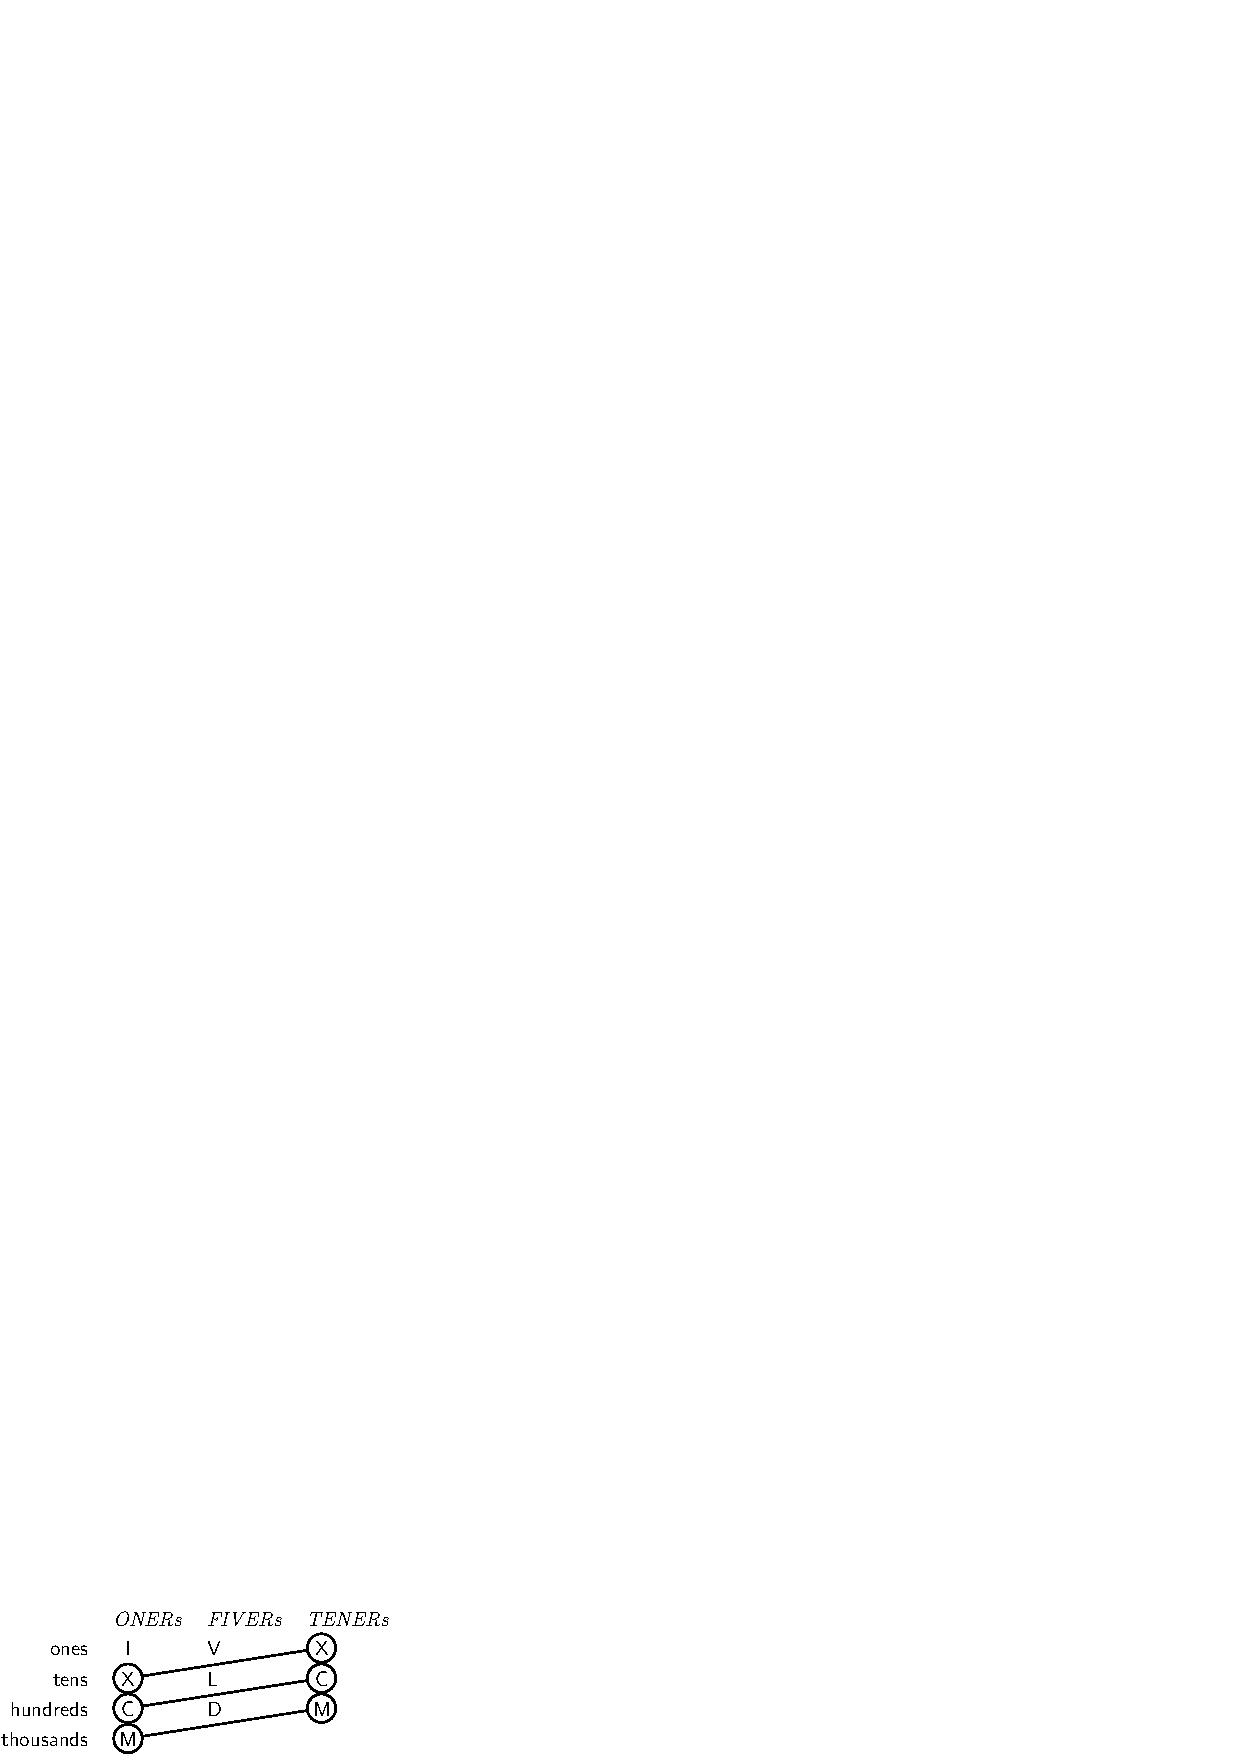
\includegraphics{inl4-1}
\bigskip

\noindent But that seems redundant. Can we avoid it? Perhaps if we try
a different model, perhaps a linear table, like this:

\bigskip
{\sf\begin{tabular}{rl}
ones      & I \\
          & V \\
tens      & X \\
          & L \\
hundreds  & C \\
          & D \\
thousands & M \\
\end{tabular}}
\bigskip

\noindent Now we can imagine that each column name (``ones,''
``tens,'' etc.) points to the ONER of that column. From there we can
also get each column's FIVER by reaching down one slot below the
current ONER, and the TENER by reaching down two slots.

It's like building an arm with three hands. We can attach it to the
ONES column, as in \Fig{fig4-8}a, or we can attach it to the tens' column,
as in \Fig{fig4-8}b, or to any power of ten.

\wepsfiga{fig4-8}{A mechanical representation: accessing the data
structure.}

%!! include Figure 4-8 here

An experienced FORTH programmer is not likely to imagine arms,
hands, or things like that. But there must be a strong mental image---the
stuff of right-brain thinking---before there's any attempt to construct the
model with code.

Beginners who are learning to think in this right-brain way might
find the following tip helpful:

%!! horizontal line
\begin{tip}
If you have trouble thinking about a conceptual model, visualize it---or
draw it---as a mechanical device.
\end{tip}
%!! horizontal line
Our table is simply an array of characters. Since a character requires only
a byte, let's make each ``slot'' one byte. We'll call the table ROMANS:

\begin{Code}
CREATE ROMANS    ( ones)  ASCII I  C,   ASCII V  C,
                 ( tens)  ASCII X  C,   ASCII L  C,
             ( hundreds)  ASCII C  C,   ASCII D  C,
            ( thousands)  ASCII M  C,
\end{Code}
Note: This use of \textbf{ASCII} requires that \textbf{ASCII} be
``\textbf{STATE}-dependent'' (see Appendix C). If you don't have \textbf{ASCII},
or if it is not state-dependent, use:

\begin{Code}
CREATE ROMANS  73 C,  86 C,  88 C,  76 C,
   67 C,  68 C,  77 C,
\end{Code}

We can select a particular symbol from the table by applying two
different offsets at the same time. One dimension represents the decimal
place: ones, tens, hundreds, etc. This dimension is made ``current,'' that
is, its state stays the same until we change it.

The other dimension represents the kind of symbol we want---ONER,
FIVER, TENER---within the current decimal column. This
dimension is incidental, that is, we'll specify which symbol we want each
time.

Let's start by implementing the ``current'' dimension. We need
some way to point to the current decimal column. Let's create a variable
called COLUMN\# (pronounced ``column-number'') and have it contain an
offset into the table:

\begin{Code}
VARIABLE COLUMN#  ( current offset)
: ONES        O COLUMN# ! ;
: TENS        2 COLUMN# ! ;
: HUNDREDS    4 COLUMN# ! ;
: THOUSANDS   6 COLUMN# ! ;
\end{Code}
Now we can find our way to any ``arm position'' by adding the contents of
COLUMN\# to the beginning address of the table, given by ROMANS:

\begin{Code}
: COLUMN  ( -- adr of column)  ROMANS  COLUMN# @  + ;
\end{Code}
Let's see if we can implement one of the words to display a symbol. We'll
start with ONER.

The thing we want to do in ONER is \textbf{EMIT} a character.

\begin{Code}
: ONER                   EMIT ;
\end{Code}
Working backward, \textbf{EMIT} requires the ASCII character on the stack.
How do we get it there? With \textbf{C@}.

\begin{Code}
: ONER                C@ EMIT ;
\end{Code}
\textbf{C@} requires the \emph{address} of the slot that contains the symbol we
want. How do we get that address?

The ONER is the first ``hand'' on the movable arm---the position
that COLUMN is already pointing to. So, the address we want is simply
the address returned by COLUMN:

\begin{Code}
: ONER   COLUMN       C@ EMIT ;
\end{Code}
Now let's write FIVER. It computes the same slot address, then adds
one to get the next slot, before fetching the symbol and emitting it:

\begin{Code}
: FIVER  COLUMN 1+    C@ EMIT ;
\end{Code}
And TENER is:

\begin{Code}
: TENER  COLUMN 2+    C@ EMIT ;
\end{Code}
These three definitions are redundant. Since the only difference between
them is the incidental offset, we can factor the incidental offset out from
the rest of the definitions:

\begin{Code}
: .SYMBOL  ( offset)  COLUMN +  C@ EMIT ;
\end{Code}
Now we can define:

\begin{Code}
: ONER    O .SYMBOL ;
: FIVER   1 .SYMBOL ;
: TENER   2 .SYMBOL ;
\end{Code}
All that remains for us to do now is to decompose our complete decimal
number into a series of decimal digits. Based on the observations we've
already made, this should be easy. Figure 4-9 shows our completed
listing.

Voila! From problem, to conceptual model, to code.

Note: this solution is not optimal. The present volume does not address
the optimization phase.

One more thought: Depending on who uses this application, we may
want to add error-checking. Fact is, the highest symbol we know is M; the
highest value we can represent is 3,999, or MMMCMXCIX.

We might redefine ROMAN as follows:

%!! I have added an IF...THEN around ABORT" Too large".
%!! Without it, it does not seem to make sense, does it?
%!! (Pg 131)
\begin{Code}
: ROMAN  ( n)
   DUP  3999 > IF  ABORT" Too large"  THEN  ROMAN ;
\end{Code}

%!! horizontal line
\blackline{2ex}
\noindent Moore:

\begin{tfquot}
There's a definite sense of rightness when you've done it right. It may be
that feeling that distinguishes FORTH from other languages, where you
never feel you've really done well. In FORTH, it's the ``Aha!'' reaction. You
want to run off and tell somebody.

Of course, nobody will appreciate it like you do.
\end{tfquot}
\blackline{1ex}
%!! horizontal line

\begin{figure*}[pppp]
\caption{Roman numerals, solved.}
\labelfig{fig4-9}
\vspace{1ex}
\setcounter{screen}{20}
\begin{Screen}
\ Roman numerals                                      8/18/83
CREATE ROMANS    ( ones)  ASCII I  C,   ASCII V  C,
                 ( tens)  ASCII X  C,   ASCII L  C,
             ( hundreds)  ASCII C  C,   ASCII D  C,
            ( thousands)  ASCII M  C,
VARIABLE COLUMN#  ( current offset)
: ONES       O COLUMN# ! ;
: TENS       2 COLUMN# ! ;
: HUNDREDS   4 COLUMN# ! ;
: THOUSANDS  6 COLUMN# ! ;

: COLUMN ( -- address of column)  ROMANS  COLUMN# @  + ;

\end{Screen}

\begin{Screen}
\ Roman numerals cont'd                               8/18/83
: .SYMBOL  ( offset -- )  COLUMN +  C@ EMIT ;
: ONER    O .SYMBOL ;
: FIVER   1 .SYMBOL ;
: TENER   2 .SYMBOL ;

: ONERS  ( # of oners -- )
   ?DUP  IF  O DO  ONER  LOOP  THEN ;
: ALMOST  ( quotient of 5 / -- )
   ONER  IF  TENER  ELSE  FIVER  THEN ;
: DIGIT  ( digit -- )
   5 /MOD  OVER  4 = IF  ALMOST  DROP  ELSE  IF FIVER THEN
   ONERS THEN ;

\end{Screen}

\begin{Screen}
\ Roman numerals cont'd                             8/18/83
: ROMAN  ( number --)  1000 /MOD  THOUSANDS DIGIT
                        100 /MOD   HUNDREDS DIGIT
                         10 /MOD       TENS DIGIT
                                       ONES DIGIT  ;

\end{Screen}
\vspace{1ex}
\label{fig-fig4-9}
\end{figure*}

\section{Summary}

In this chapter we've learned to develop a single component, starting
first with deciding on its syntax, then proceeding with determining its
algorithm(s) and data structure(s), and concluding with an implementation
in FORTH.

With this chapter we complete our discussion of design. The remainder
of the book will discuss style and programming techniques.

\section{References}

%!! the ordered list thing again
\begin{enumerate}
\item G. Polya, \emph{How To Solve It: A New Aspect of Mathematical Method},
   (Princeton, New Jersey, Princeton University Press).
%!! (C) should be a nicer copyright sign
\item Leslie A. Hart, \emph{How the Brain Works}, \copyright{} 1975 by Leslie A. Hart,
   (New York, Basic Books, Inc., 1975).
\item Evan Rosen, ``High Speed, Low Memory Consumption Structures,'' 1982
   \emph{FORML Conference Proceedings}, p. 191.
\item Michael Stolowitz, ``A Compiler for Programmable Logic in FORTH,'' 1982
   \emph{FORML Conference Proceedings}, p. 257.
\end{enumerate}

\section{For Further Thinking}

Design the components and describe the algorithm(s) necessary to simulate
shuffling a deck of cards. Your algorithm will produce an array of
numbers, 0--51, arranged in random order.

The special constraint of this problem, of course, is that no one card
may appear twice in the array.

You may assume you have a random-number generator called
CHOOSE. It's stack argument is ``n''; it produces a random number
between zero and n-1 inclusive. (See the Handy Hint, Chapter Ten,
\emph{Starting FORTH}.)

Can you design the card-shuffling algorithm so that it avoids the
time-consuming burden of checking some undetermined number of slots
on each pass of the loop? Can you do so using only the one array?
